\paragraph{QuizziPedia::Front-End::Directives::ImageInTheQuestionDirective}
\begin{figure} [ht]
	\centering
	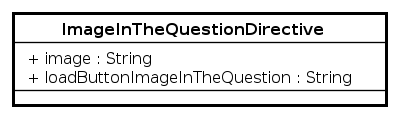
\includegraphics[scale=0.80]{UML/Classi/Front-End/QuizziPedia_Front-end_ImageInTheQuestionDirective.png}
	\caption{QuizziPedia::Front-End::Directives:ImageInTheQuestionDirective}
\end{figure} \FloatBarrier
\begin{itemize}
	\item \textbf{Descrizione}: \textit{directive\ped{G}} contenente i componenti grafici per l'inserimento dell'immagine nella creazione delle domande;
	\item \textbf{Utilizzo}: permette di per inserire un'immagine in una domanda;
	\item \textbf{Relazioni con altre classi}:
	\begin{itemize}
		\item \textbf{OUT \texttt{TrueFalseQuestionsView}}: \textit{view\ped{G}} contenente i campi per creare una domanda vero/falso; 
		\item \textbf{OUT \texttt{MultipleQuestionsView}}:  \textit{view\ped{G}} contenente i campi per creare una domanda a risposta multipla; 
		\item \textbf{OUT \texttt{ImagesSortingQuestionsView}}: \textit{view\ped{G}} contenente i campi per creare una domanda a ordinamento immagini;
		\item \textbf{OUT \texttt{ClickableAreaQuestionsView}}:  \textit{view\ped{G}} contenente i campi per creare una domanda ad area cliccabile.
	\end{itemize}
	\item \textbf{Attributi}:
	\begin{itemize}
		\item \texttt{+ image: String} \\ Attributo contenete l'URL dell'immagine caricata dall'utente;
		\item \texttt{+ loadButtonImageInTheQuestion: String} \\ Attributo che viene utilizzato per visualizzare la giusta traduzione della \textit{label\ped{G}} per il bottone di caricamento dell'immagine, in italiano o in inglese. 
	\end{itemize}
\end{itemize}